
\section[Work Flows]{Work Flows}
\label{sec:work_flows}
\addcontentsline{toc}{section}{\thesection. Work Flows}

{\color{red} \bf Warning:}
All work flows are supposed to be run under batch mode and Unix-like systems
due to performance.

\pkg{cubfits} is tested and built with some useful work flows,
including
\begin{enumerate}
\item \code{simu} for simulation studies,
\item \code{wphi} for sequences with expression levels and measurement errors,
      and
\item \code{wophi} for sequences without expression levels.
\end{enumerate}
Upon the \pkg{cubfits} package release,
we also share these work flows as templates which may be useful for further
researches. A quick way to obtain a default work flow is via an internal
function call \code{cubfits::cp.workflow()}. There are currently three work
flows built within this call.
Note that all of these are only tested privately under the Linux system,
merely served as templates, none of them are checked by CRAN.

The work flows are stored in the package directory
\code{cubfits/inst/workflow/} and installed in
\code{$\{R_HOME\}/library/cubfits/workflow/}. Therefore, execute the
follow script can regenerate those work flows in three directories
\code{./01-simu/}, \code{./02-wphi/}, and \code{./03-wophi/}.
\begin{Command}
$ mkdir 01-simu
$ cd 01-simu/
$ Rscript -e "cubfits::cp.workflow('simu')"
$ cd ../
$ mkdir 02-wphi
$ cd 02-wphi/
$ Rscript -e "cubfits::cp.workflow('wphi')"
$ cd ../
$ mkdir 03-wophi
$ cd 03-wophi/
$ Rscript -e "cubfits::cp.workflow('wophi')"
$ cd ../
\end{Command}
Note that a work flow is mainly coded in shell script and sequentially
executes analyses via several shell commands and \proglang{R} scripts. The
analysis \proglang{R} scripts are managed and stored in
\code{cubfits/inst/workflow/code/} and installed in
\code{$\{R_HOME\}/library/cubfits/workflow/code/}. Those are served as
templates and can be altered by users (copy scripts to local directory
and change to what they should be.)

After regenerating those work flows,
three shell scripts and one \proglang{R} script are created
within each directories as
\begin{itemize}
\item \code{run_0.sh} is to create subdirectories for storages,
\item \code{run_1.sh} is the main script of analysis,\footnote{
This may require up to 30 cores and may take a few hours to finish
depending on number of sequences. Please do some test and adjust
this file and \code{00-set\_env.r} accordingly before a hero run.
}
\item \code{run_2.sh} is for post processes, and
\item \code{00-set_env.r} is the \proglang{R} script for configurations.
\end{itemize}
For \code{simu} work flow, one can execute sequentially those shell scripts
(\code{run_*.sh})
without further changes, and may learn to adjust scripts for further studies.
For \code{wphi} and \code{wophi} work flows, one needs to provide genome
sequences (e.g. \code{./02-wphi/param/genome.fasta})
and expression data (e.g. \code{./02-wphi/param/genome.phi.tsv})
by replacing files.

Examples of post processes (\code{run_2.sh}) from \code{simu} work flow
are given in Figure~\ref{fig:prxy}. The plots are from files
\code{./01-simu/all.out/plot/prxy_roc_ad_fits_pm_5k-10k.pdf} and \\
\code{./01-simu/all.out/plot/prxy_roc_ad_appr_pm_5k-10k.pdf}.
\begin{figure}[ht]
\centering
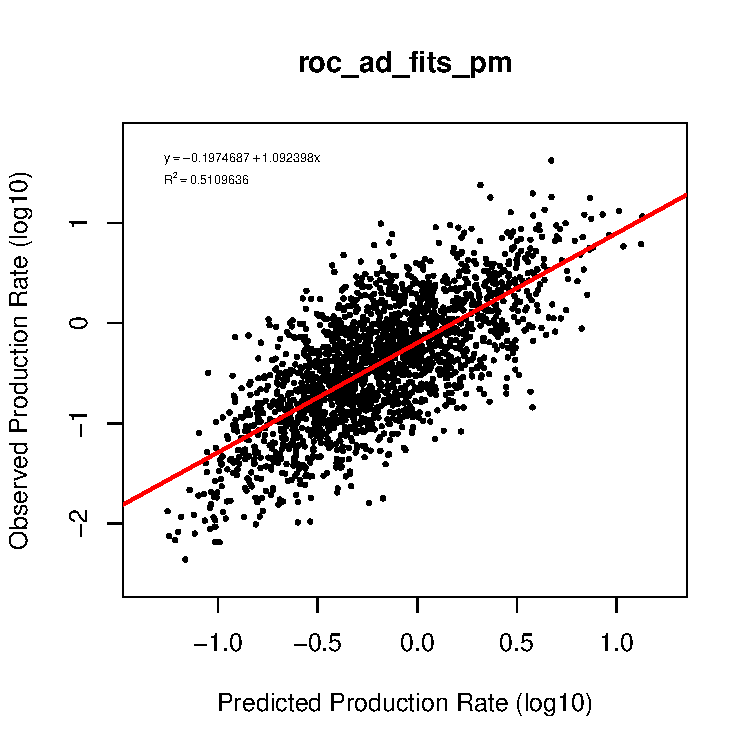
\includegraphics[width=2.75in]{cubfits-include/figure/prxy_roc_ad_fits_pm_5k-10k}
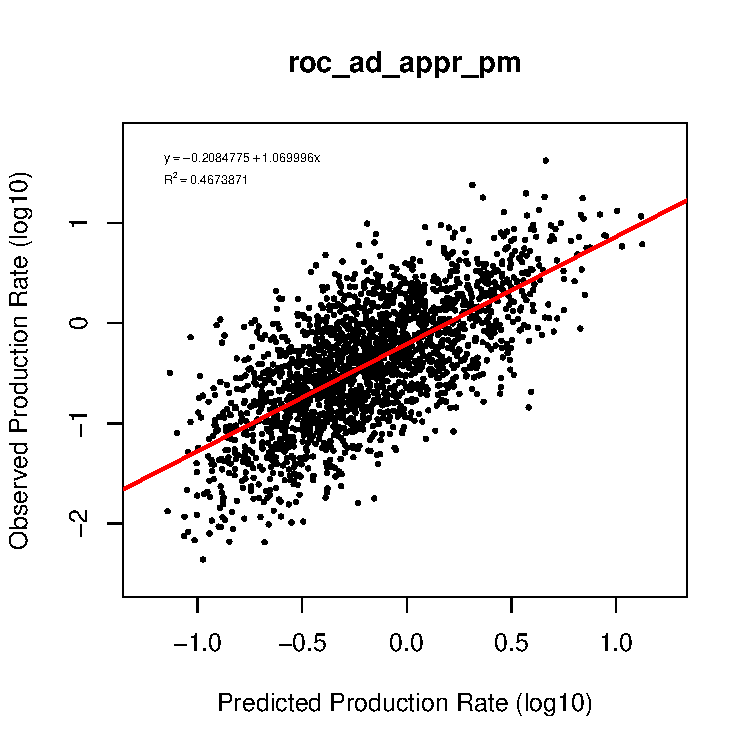
\includegraphics[width=2.75in]{cubfits-include/figure/prxy_roc_ad_appr_pm_5k-10k}
\caption{The left plot is predicted expression (MCMC posterior mean of expected
expression) from model fits against observed
expression (with measurement errors). In the right plot, the predicted
expression is approximated from a simulation (no model fits.)}
\label{fig:prxy}
\end{figure}
